\loesung{
\begin{enumerate}[a)]
\item Pseudocode of \texttt{get\_bounds()}

\begin{algorithm}[h]
\caption{\texttt{get\_bounds()}}
\begin{algorithmic}[1]
\Require \texttt{X}: input data 
\Require \texttt{s}: index of features for calculating ALE
\Require \texttt{n\_intervals}: number of intervals 
\State \texttt{x\_s} $\gets$ s-th column of \texttt{X}
\State \texttt{x\_s\_min} $\gets$ min value of \texttt{x\_s}
\State \texttt{x\_s\_max} $\gets$ max value of \texttt{x\_s}
\State \textbf{return} equidistant sequence of \texttt{n\_intervals + 1} grid points between \texttt{x\_s\_min} and \texttt{x\_s\_max}
\end{algorithmic}
\end{algorithm}

% \lstinputlisting{"rsrc/get_bounds().R"}

\item Pseudocode of \texttt{calculate\_ale()}

\begin{algorithm}[h]
\caption{\texttt{calculate\_ale()}}
\begin{algorithmic}[1]
\Require \texttt{model} : Classifier 
\Require \texttt{X}: input data 
\Require \texttt{s}: index of feature for calculating ALE
\Require \texttt{n\_intervals}: number of intervals 
\Require \texttt{centered}: whether to return centered or uncentered ALE
\State \texttt{bounds} $\gets$ \texttt{get\_bounds}(\texttt{X}, \texttt{s}, \texttt{n\_intervals})
\State \texttt{lowerbound} $\gets$ lower interval bounds
\State \texttt{upperbound} $\gets$ upper interval bounds
\State \texttt{result} $\gets$ \{\}
\For{\texttt{i1} in \texttt{lowerbound} \& \texttt{i2} in \texttt{upperbound}}
\State \texttt{idx} $\gets$ ids of datapoints of \texttt{X} $\in$ (\texttt{i1}, \texttt{i2}] \Comment{for first interval [\texttt{i1}, \texttt{i2}]}
\If{idx = $\emptyset$} diff $\gets$ 0
\ElsIf {idx $\neq \emptyset$}
\State \texttt{X\_min} $\gets$ $\texttt{X[idx,]}$ with feature values of $s$ replaced by $i1$
\State \texttt{X\_max} $\gets$ $\texttt{X[idx,]}$ with feature values of $s$ replaced by $i2$
\State \texttt{y\_min} $\gets$ \texttt{model} predictions of \texttt{X\_min}
\State \texttt{y\_max} $\gets$ \texttt{model} predictions of \texttt{X\_max}
\State \texttt{diff} $\gets$ \texttt{y\_max} - \texttt{y\_min} 
\EndIf
\State \texttt{results} $\gets$ \{\texttt{results}, mean of \texttt{diff}\}
\EndFor
\State \texttt{uncentered\_ale} $\gets$ cumulative sum of \texttt{result}
\If{\texttt{centered}} \texttt{centered\_ale} $\gets$ \texttt{uncentered\_ale} - (mean of \texttt{uncentered\_ale}) 
\EndIf
\State \textbf{return}  \texttt{bounds} and either \texttt{uncentered\_ale} or \texttt{centered\_ale}
\end{algorithmic}
\end{algorithm}

%\lstinputlisting{"rsrc/calculate_ale().R"}

\item Pseudocode of  \texttt{prepare\_ale()}

\begin{algorithm}[h]
\caption{\texttt{prepare\_ale()}}
\begin{algorithmic}[1]
\Require \texttt{model} : Classifier 
\Require \texttt{X}: input data 
\Require \texttt{s}: index of feature for calculating ALE
\Require \texttt{n\_intervals}: number of intervals 
\Require \texttt{centered}: whether to return centered or uncentered ALE
\State \texttt{bounds, y} $\gets$ \texttt{prepare\_ale}(\texttt{X}, \texttt{s}, \texttt{n\_intervals}, \texttt{centered})
\State \texttt{lowerbound} $\gets$ lower interval bounds
\State \texttt{upperbound} $\gets$ upper interval bounds
\State \texttt{x} $\gets$ center of each interval (middle of \texttt{lowerbound} and \texttt{upperbound})
\State \textbf{return}  \texttt{x} and \texttt{y}
\end{algorithmic}
\end{algorithm}

%\lstinputlisting{"rsrc/prepare_ale().R"}

%\item Example:
%\lstinputlisting{"rsrc/example_ale.R"}

%\begin{center}
%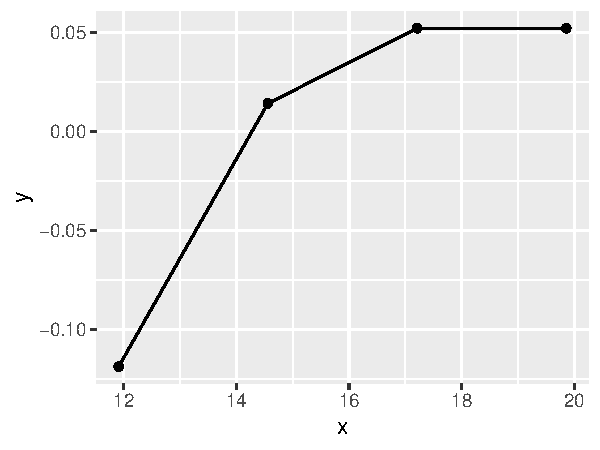
\includegraphics[width=\maxwidth]{figure/example_ale.pdf}
%\end{center}

\end{enumerate}
}